\subsection{Mission}

Au cours de mon stage, j'ai entrepris diverses missions au sein de l'association dans le but de mener à bien le projet qui m'a été confié.

Initialement, je vais détailler en profondeur le projet qui m'a été attribué, puis je vais fournir des explications approfondies sur les différentes tâches entreprises pour la réalisation réussie de ce projet.

\subsubsection{Le projet}

Le projet consiste en la création d'une application interne à l'école CY~Tech, visant à améliorer la communication des associations étudiantes concernant les événements qu'elles organisent. Cette application offre aux étudiants la possibilité de s'inscrire aisément aux événements et de rester informés plus facilement de ce qui se passe autour d'eux.

Le projet est subdivisé en deux sous-projets : le développement d'une application web et la création d'une API.

L'application web fait office d'interface graphique entre l'utilisateur et l'API, assurant la liaison entre la base de données et l'interface utilisateur. Nous avons fait le choix de diviser le projet en deux parties distinctes pour garantir une maintenance optimale des applications et permettre à plusieurs applications web de bénéficier de ce service.

Plusieurs fonctionnalités essentielles sont prévues pour les applications :
\begin{itemize}
	\item Création et gestion de comptes utilisateurs ;
	\item Abonnement aux associations ;
	\item Participation aux événements ;
	\item Création d'événements ponctuels ou récurrents.
\end{itemize}

Il est impératif que les applications soient hautement sécurisées, tout en garantissant une maintenance aisée et une extensibilité optimale.

Cependant, la réalisation de ces objectifs est soumise à plusieurs contraintes spécifiques liées au développement des applications.

Concernant l'application web, il est impératif qu'elle soit conçue selon le concept de Single Page Application (SPA), offrant ainsi une expérience utilisateur fluide et réactive. Cette approche permettra de réduire les temps de chargement en ne rechargeant que les éléments nécessaires à l'écran, améliorant ainsi l'efficacité et la rapidité de l'application.

En ce qui concerne l'API, une exigence cruciale est sa réactivité. L'API devra être en mesure de gérer simultanément de multiples requêtes et d'y répondre efficacement, tout en maintenant des temps de réponse courts. Cette réactivité est essentielle pour garantir une expérience utilisateur optimale, même en périodes de pic d'utilisation.

Ces contraintes, bien que complexes, contribuent à l'élaboration d'applications performantes et conviviales, conformes aux besoins et aux attentes des utilisateurs.


\subsubsection{Détails}

\paragraph{Les comptes utilisateurs}
~~\\

Posséder un compte utilisateur constitue un élément clé dans l'expérience d'utilisation d'une application. Il permet de personnaliser les préférences de l'utilisateur et de stocker des informations en lien avec le contenu proposé par l'application. Cependant, il est impératif de garantir une sécurisation rigoureuse de l'authentification afin d'éviter tout accès non autorisé à un compte.

Dans le souci de renforcer la sécurité de notre système d'authentification, notre choix s'est porté sur Keycloak, une plateforme spécialisée dédiée à cette fin. Keycloak exploite le protocole OpenID Connect (OIDC), qui assure un processus d'authentification à la fois sûr et robuste.

OpenID Connect (OIDC) repose sur OAuth 2.0 et se positionne comme un protocole d'authentification conçu spécifiquement pour sécuriser les échanges entre applications et services en ligne. Il permet à un utilisateur de s'authentifier au sein d'une application en utilisant son identité issue d'un fournisseur d'identité tiers, comme Keycloak. L'utilisation de jetons d'authentification renforce le niveau de sécurité, contribuant ainsi à la fiabilité et à l'efficacité du processus.

La gestion des jetons d'authentification au sein de Keycloak s'articule comme suit : lorsqu'un utilisateur se connecte, Keycloak génère un jeton d'authentification. L'utilisateur reçoit ce jeton qui est ensuite transmis à chaque requête vers l'application API. Avant l'exécution de la requête, Keycloak vérifie l'authentification de l'utilisateur ainsi que ses droits pour effectuer la demande. Si les conditions sont satisfaites, la requête est exécutée. Une caractéristique avantageuse des jetons générés par Keycloak est leur expiration, prévenant ainsi la rétention d'un jeton inutilisé sur l'appareil de l'utilisateur pendant une période prolongée. Par ailleurs, Keycloak adopte le concept de Single Sign-On (SSO), ce qui signifie qu'une fois qu'un utilisateur s'est authentifié auprès d'une application, aucune nouvelle connexion n'est requise lorsqu'il accède à d'autres applications sécurisées par Keycloak au sein de la même session.

En somme, l'utilisation du protocole OIDC via Keycloak pour la gestion des jetons d'authentification renforce la sécurité et la convivialité de l'authentification pour les applications et les utilisateurs. Cette approche permet d'établir un environnement centralisé et sécurisé pour l'authentification, englobant l'ensemble des applications développées au sein de la Corpauration.

\begin{figure}
	\centering
	\begin{subfigure}{.45\textwidth}
		\centering
		
\includegraphics[width=0.40\textwidth]{assets/keycloak.png}
		\subcaption{Keycloak}
		\label{fig:keycloak}
	\end{subfigure}
	\begin{subfigure}{.45\textwidth}
		\centering
		\includegraphics[width=0.40\textwidth]{assets/openid.png}
		\subcaption{OpenID}
		\label{fig:openid}
	\end{subfigure}
	\caption{Technologies utilisées pour l'authentification}
\end{figure}

\paragraph{Abonnements aux associations}
~~\\

Étant donné que chaque association possède ses propres particularités, il est prévu de mettre en place un système d'abonnement personnalisé. Ce système permettra aux étudiants de sélectionner les associations qui les intéressent particulièrement. En conséquence, les utilisateurs disposeront d'une expérience utilisateur améliorée, en accédant plus aisément aux événements susceptibles de les intéresser.

\paragraph{Participation aux événements}
~~\\

La possibilité de participer aux événements via l'application présente deux avantages majeurs, à la fois pour les étudiants et pour les associations.

Nous avons constaté qu'il existe un certain désintérêt lorsque les étudiants doivent cliquer sur un lien externe, comme un formulaire Google Form, pour s'inscrire à un événement. Ce processus engendre souvent une baisse du taux de participation. Afin de pallier cette problématique, nous avons opté pour une simplification du processus d'inscription en centralisant toutes les étapes au sein de l'application. De cette manière, il devient plus aisé pour les étudiants de s'inscrire en utilisant les informations déjà enregistrées dans la base de données. Les associations bénéficieront d'une augmentation du nombre d'inscrits et disposeront d'un onglet dédié pour consulter la liste complète des participants. Du côté des étudiants, ils auront un accès direct aux événements auxquels ils se sont inscrits, ainsi que la possibilité de définir des rappels pour ne manquer aucun événement.

Cette approche permet donc de simplifier le processus d'inscription, d'augmenter la participation des étudiants aux événements et d'optimiser la gestion des inscriptions pour les associations.


\paragraph{Création d'événements}
~~\\

La création d'événements constitue la fonctionnalité centrale de l'application. L'objectif est de fournir une personnalisation maximale lors de la création d'événements. Cela inclut la flexibilité de renseigner certains champs selon les besoins, la faculté de créer des événements récurrents et la possibilité de procéder à des modifications en toute liberté.

\paragraph{L'application web}
~~\\

Pour mettre en œuvre toutes ces fonctionnalités de manière conviviale, l'utilisation d'une interface graphique s'impose. Ainsi, nous avons pris la décision de développer une application web pour permettre un accès aisé à l'ensemble des fonctionnalités.

Pour cela, nous avons opté pour l'utilisation du célèbre framework JavaScript Vue, conjugué à la bibliothèque open-source de composants Vuetify.

Vue est un framework JavaScript progressif et performant destiné à la création d'interfaces utilisateur interactives et dynamiques. Il simplifie le processus de développement en offrant une structure organisée pour la construction d'applications web grâce à la composition de composants réutilisables. Vue met l'accent sur la réactivité des données, permettant ainsi les changements dans l'état de l'application à se refléter automatiquement dans l'interface utilisateur, sans nécessiter de manipulations directes du DOM.

De son côté, Vuetify est une bibliothèque de composants visuels conçue spécifiquement pour Vue.js. Elle vise à simplifier la création d'interfaces utilisateur esthétiques et réactives. Vuetify met à disposition une gamme complète de composants préconçus, tels que des boutons, des barres de navigation, des cartes, et bien plus encore. Ces composants peuvent être intégrés en toute simplicité dans des projets Vue, accélérant ainsi le processus de développement tout en assurant une cohérence visuelle à travers l'application. Grâce à Vuetify, il devient possible de concevoir rapidement des interfaces modernes et attrayantes sans nécessiter la création de chaque élément visuel à partir de zéro.

L'application web ne communiquera pas directement avec la base de données, mais plutôt avec une API dédiée qui assurera l'ensemble des échanges avec la base de données.

\begin{figure}[h]
	\centering
	\begin{subfigure}{.45\textwidth}
		\centering
		
\includegraphics[width=0.40\textwidth]{assets/vue.png}
		\subcaption{Vue}
		\label{fig:vue}
	\end{subfigure}
	\begin{subfigure}{.45\textwidth}
		\centering
		
\includegraphics[width=0.40\textwidth]{assets/vuetify.png}
		\subcaption{Vuetify}
		\label{fig:vuetify}
	\end{subfigure}
	\caption{Technologies utilisées pour l'application web}
\end{figure}

\paragraph{L'API}
~~\\

L'API (Interface de Programmation d'Application) agit comme un pont de connexion entre deux logiciels distincts. Dans le cadre de notre projet, l'API jouera le rôle d'intermédiaire, connectant l'application web (interface utilisateur) à la base de données. Bien qu'il soit possible de relier directement l'application web à la base de données, cette approche complexifie le développement de l'interface, entraînant une application moins maintenable et moins sécurisée.

Une autre motivation pour l'utilisation d'une API réside dans sa capacité à être partagée entre plusieurs applications web. Nous envisageons d'utiliser cette même API à l'avenir pour synchroniser les événements auxquels les étudiants participent avec leur emploi du temps grâce à l'application Cyrel. Cette dernière, également développée par la Corpauration, a pour objectif de fournir un emploi du temps moderne pour faciliter le suivi des cours.

\begin{figure}[h]
	\centering
	\begin{subfigure}{.45\textwidth}
		\centering
		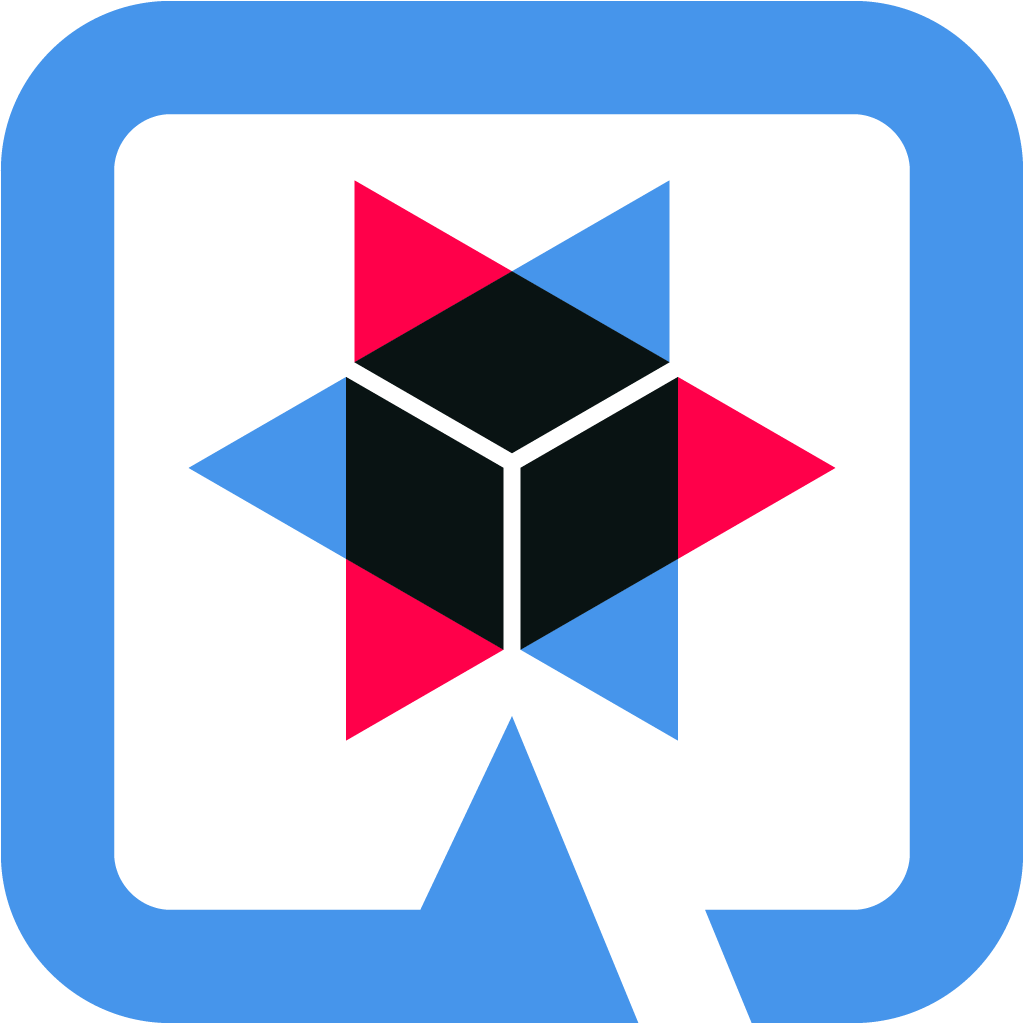
\includegraphics[width=0.40\textwidth]{assets/quarkus.png}
		\subcaption{Quarkus}
		\label{fig:quarkus}
	\end{subfigure}
	\begin{subfigure}{.45\textwidth}
		\centering
		
\includegraphics[width=0.40\textwidth]{assets/hibernate.png}
		\subcaption{Hibernate}
		\label{fig:openid}
	\end{subfigure}
	\caption{Technologies utilisées pour l'API}
\end{figure}

